\documentclass[twoside]{book}

% Packages required by doxygen
\usepackage{fixltx2e}
\usepackage{calc}
\usepackage{doxygen}
\usepackage[export]{adjustbox} % also loads graphicx
\usepackage{graphicx}
\usepackage[utf8]{inputenc}
\usepackage{makeidx}
\usepackage{multicol}
\usepackage{multirow}
\PassOptionsToPackage{warn}{textcomp}
\usepackage{textcomp}
\usepackage[nointegrals]{wasysym}
\usepackage[table]{xcolor}

% Font selection
\usepackage[T1]{fontenc}
\usepackage[scaled=.90]{helvet}
\usepackage{courier}
\usepackage{amssymb}
\usepackage{sectsty}
\renewcommand{\familydefault}{\sfdefault}
\allsectionsfont{%
  \fontseries{bc}\selectfont%
  \color{darkgray}%
}
\renewcommand{\DoxyLabelFont}{%
  \fontseries{bc}\selectfont%
  \color{darkgray}%
}
\newcommand{\+}{\discretionary{\mbox{\scriptsize$\hookleftarrow$}}{}{}}

% Page & text layout
\usepackage{geometry}
\geometry{%
  a4paper,%
  top=2.5cm,%
  bottom=2.5cm,%
  left=2.5cm,%
  right=2.5cm%
}
\tolerance=750
\hfuzz=15pt
\hbadness=750
\setlength{\emergencystretch}{15pt}
\setlength{\parindent}{0cm}
\setlength{\parskip}{3ex plus 2ex minus 2ex}
\makeatletter
\renewcommand{\paragraph}{%
  \@startsection{paragraph}{4}{0ex}{-1.0ex}{1.0ex}{%
    \normalfont\normalsize\bfseries\SS@parafont%
  }%
}
\renewcommand{\subparagraph}{%
  \@startsection{subparagraph}{5}{0ex}{-1.0ex}{1.0ex}{%
    \normalfont\normalsize\bfseries\SS@subparafont%
  }%
}
\makeatother

% Headers & footers
\usepackage{fancyhdr}
\pagestyle{fancyplain}
\fancyhead[LE]{\fancyplain{}{\bfseries\thepage}}
\fancyhead[CE]{\fancyplain{}{}}
\fancyhead[RE]{\fancyplain{}{\bfseries\leftmark}}
\fancyhead[LO]{\fancyplain{}{\bfseries\rightmark}}
\fancyhead[CO]{\fancyplain{}{}}
\fancyhead[RO]{\fancyplain{}{\bfseries\thepage}}
\fancyfoot[LE]{\fancyplain{}{}}
\fancyfoot[CE]{\fancyplain{}{}}
\fancyfoot[RE]{\fancyplain{}{\bfseries\scriptsize Generated by Doxygen }}
\fancyfoot[LO]{\fancyplain{}{\bfseries\scriptsize Generated by Doxygen }}
\fancyfoot[CO]{\fancyplain{}{}}
\fancyfoot[RO]{\fancyplain{}{}}
\renewcommand{\footrulewidth}{0.4pt}
\renewcommand{\chaptermark}[1]{%
  \markboth{#1}{}%
}
\renewcommand{\sectionmark}[1]{%
  \markright{\thesection\ #1}%
}

% Indices & bibliography
\usepackage{natbib}
\usepackage[titles]{tocloft}
\setcounter{tocdepth}{3}
\setcounter{secnumdepth}{5}
\makeindex

% Hyperlinks (required, but should be loaded last)
\usepackage{ifpdf}
\ifpdf
  \usepackage[pdftex,pagebackref=true]{hyperref}
\else
  \usepackage[ps2pdf,pagebackref=true]{hyperref}
\fi
\hypersetup{%
  colorlinks=true,%
  linkcolor=blue,%
  citecolor=blue,%
  unicode%
}

% Custom commands
\newcommand{\clearemptydoublepage}{%
  \newpage{\pagestyle{empty}\cleardoublepage}%
}

\usepackage{caption}
\captionsetup{labelsep=space,justification=centering,font={bf},singlelinecheck=off,skip=4pt,position=top}

%===== C O N T E N T S =====

\begin{document}

% Titlepage & ToC
\hypersetup{pageanchor=false,
             bookmarksnumbered=true,
             pdfencoding=unicode
            }
\pagenumbering{roman}
\begin{titlepage}
\vspace*{7cm}
\begin{center}%
{\Large My Project }\\
\vspace*{1cm}
{\large Generated by Doxygen 1.8.11}\\
\end{center}
\end{titlepage}
\clearemptydoublepage
\tableofcontents
\clearemptydoublepage
\pagenumbering{arabic}
\hypersetup{pageanchor=true}

%--- Begin generated contents ---
\chapter{File Index}
\section{File List}
Here is a list of all files with brief descriptions\+:\begin{DoxyCompactList}
\item\contentsline{section}{\hyperlink{Lab1_8c}{Lab1.\+c} }{\pageref{Lab1_8c}}{}
\end{DoxyCompactList}

\chapter{File Documentation}
\hypertarget{UniqueFactorization_8cpp}{}\section{Unique\+Factorization.\+cpp File Reference}
\label{UniqueFactorization_8cpp}\index{Unique\+Factorization.\+cpp@{Unique\+Factorization.\+cpp}}
{\ttfamily \#include $<$iostream$>$}\\*
Include dependency graph for Unique\+Factorization.\+cpp\+:
\nopagebreak
\begin{figure}[H]
\begin{center}
\leavevmode
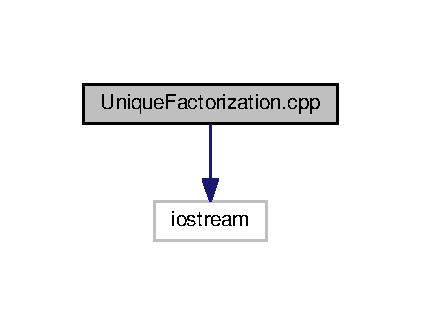
\includegraphics[width=202pt]{UniqueFactorization_8cpp__incl}
\end{center}
\end{figure}
\subsection*{Functions}
\begin{DoxyCompactItemize}
\item 
void \hyperlink{UniqueFactorization_8cpp_abb73faf2143cbadfd2cc32379ec25f72}{print\+Array} (int p\mbox{[}$\,$\mbox{]}, int n)
\item 
void \hyperlink{UniqueFactorization_8cpp_ae8ed10ed0cebde2adab2a54d4bd60730}{print\+All\+Unique\+Parts} (int n)
\item 
int \hyperlink{UniqueFactorization_8cpp_ae66f6b31b5ad750f1fe042a706a4e3d4}{main} ()
\end{DoxyCompactItemize}


\subsection{Function Documentation}
\index{Unique\+Factorization.\+cpp@{Unique\+Factorization.\+cpp}!main@{main}}
\index{main@{main}!Unique\+Factorization.\+cpp@{Unique\+Factorization.\+cpp}}
\subsubsection[{\texorpdfstring{main()}{main()}}]{\setlength{\rightskip}{0pt plus 5cm}int main (
\begin{DoxyParamCaption}
{}
\end{DoxyParamCaption}
)}\hypertarget{UniqueFactorization_8cpp_ae66f6b31b5ad750f1fe042a706a4e3d4}{}\label{UniqueFactorization_8cpp_ae66f6b31b5ad750f1fe042a706a4e3d4}

\begin{DoxyCode}
62 \{
63     cout << \textcolor{stringliteral}{"All Unique Partitions of 2 \(\backslash\)n"};
64     \hyperlink{UniqueFactorization_8cpp_ae8ed10ed0cebde2adab2a54d4bd60730}{printAllUniqueParts}(2);
65  
66     cout << \textcolor{stringliteral}{"\(\backslash\)nAll Unique Partitions of 3 \(\backslash\)n"};
67     \hyperlink{UniqueFactorization_8cpp_ae8ed10ed0cebde2adab2a54d4bd60730}{printAllUniqueParts}(3);
68  
69     cout << \textcolor{stringliteral}{"\(\backslash\)nAll Unique Partitions of 4 \(\backslash\)n"};
70     \hyperlink{UniqueFactorization_8cpp_ae8ed10ed0cebde2adab2a54d4bd60730}{printAllUniqueParts}(4);
71  
72     \textcolor{keywordflow}{return} 0;
73 \}\end{DoxyCode}


Here is the call graph for this function\+:
\nopagebreak
\begin{figure}[H]
\begin{center}
\leavevmode
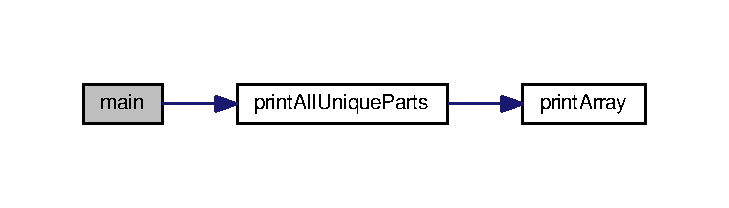
\includegraphics[width=350pt]{UniqueFactorization_8cpp_ae66f6b31b5ad750f1fe042a706a4e3d4_cgraph}
\end{center}
\end{figure}


\index{Unique\+Factorization.\+cpp@{Unique\+Factorization.\+cpp}!print\+All\+Unique\+Parts@{print\+All\+Unique\+Parts}}
\index{print\+All\+Unique\+Parts@{print\+All\+Unique\+Parts}!Unique\+Factorization.\+cpp@{Unique\+Factorization.\+cpp}}
\subsubsection[{\texorpdfstring{print\+All\+Unique\+Parts(int n)}{printAllUniqueParts(int n)}}]{\setlength{\rightskip}{0pt plus 5cm}void print\+All\+Unique\+Parts (
\begin{DoxyParamCaption}
\item[{int}]{n}
\end{DoxyParamCaption}
)}\hypertarget{UniqueFactorization_8cpp_ae8ed10ed0cebde2adab2a54d4bd60730}{}\label{UniqueFactorization_8cpp_ae8ed10ed0cebde2adab2a54d4bd60730}

\begin{DoxyCode}
13 \{
14     \textcolor{keywordtype}{int} p[n]; \textcolor{comment}{// An array to store a partition}
15     \textcolor{keywordtype}{int} k = 0; \textcolor{comment}{// Index of last element in a partition}
16     p[k] = n; \textcolor{comment}{// Initialize first partition as number itself}
17  
18     \textcolor{comment}{// This loop first prints current partition, then generates next}
19     \textcolor{comment}{// partition. The loop stops when the current partition has all 1s}
20     \textcolor{keywordflow}{while} (\textcolor{keyword}{true})
21     \{
22         \textcolor{comment}{// print current partition}
23         \hyperlink{UniqueFactorization_8cpp_abb73faf2143cbadfd2cc32379ec25f72}{printArray}(p, k + 1);
24  
25         \textcolor{comment}{// Generate next partition}
26  
27         \textcolor{comment}{// Find the rightmost non-one value in p[]. Also, update the}
28         \textcolor{comment}{// rem\_val so that we know how much value can be accommodated}
29         \textcolor{keywordtype}{int} rem\_val = 0;
30         \textcolor{keywordflow}{while} (k >= 0 && p[k] == 1)
31         \{
32             rem\_val += p[k];
33             k--;
34         \}
35  
36         \textcolor{comment}{// if k < 0, all the values are 1 so there are no more partitions}
37         \textcolor{keywordflow}{if} (k < 0)
38             \textcolor{keywordflow}{return};
39  
40         \textcolor{comment}{// Decrease the p[k] found above and adjust the rem\_val}
41         p[k]--;
42         rem\_val++;
43  
44         \textcolor{comment}{// If rem\_val is more, then the sorted order is violeted.  Divide}
45         \textcolor{comment}{// rem\_val in differnt values of size p[k] and copy these values at}
46         \textcolor{comment}{// different positions after p[k]}
47         \textcolor{keywordflow}{while} (rem\_val > p[k])
48         \{
49             p[k + 1] = p[k];
50             rem\_val = rem\_val - p[k];
51             k++;
52         \}
53  
54         \textcolor{comment}{// Copy rem\_val to next position and increment position}
55         p[k + 1] = rem\_val;
56         k++;
57     \}
58 \}
\end{DoxyCode}


Here is the call graph for this function\+:
\nopagebreak
\begin{figure}[H]
\begin{center}
\leavevmode
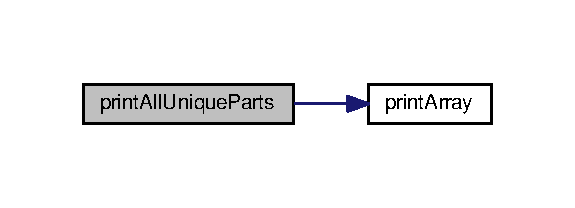
\includegraphics[width=276pt]{UniqueFactorization_8cpp_ae8ed10ed0cebde2adab2a54d4bd60730_cgraph}
\end{center}
\end{figure}


\index{Unique\+Factorization.\+cpp@{Unique\+Factorization.\+cpp}!print\+Array@{print\+Array}}
\index{print\+Array@{print\+Array}!Unique\+Factorization.\+cpp@{Unique\+Factorization.\+cpp}}
\subsubsection[{\texorpdfstring{print\+Array(int p[], int n)}{printArray(int p[], int n)}}]{\setlength{\rightskip}{0pt plus 5cm}void print\+Array (
\begin{DoxyParamCaption}
\item[{int}]{p\mbox{[}$\,$\mbox{]}, }
\item[{int}]{n}
\end{DoxyParamCaption}
)}\hypertarget{UniqueFactorization_8cpp_abb73faf2143cbadfd2cc32379ec25f72}{}\label{UniqueFactorization_8cpp_abb73faf2143cbadfd2cc32379ec25f72}

\begin{DoxyCode}
6 \{
7     \textcolor{keywordflow}{for} (\textcolor{keywordtype}{int} i = 0; i < n; i++)
8         cout << p[i] << \textcolor{stringliteral}{" "};
9     cout << endl;
10 \}
\end{DoxyCode}

%--- End generated contents ---

% Index
\backmatter
\newpage
\phantomsection
\clearemptydoublepage
\addcontentsline{toc}{chapter}{Index}
\printindex

\end{document}
